\documentclass[a4paper, 11pt]{article}

\usepackage{natbib}
\bibliographystyle{agsm}
\setcitestyle{authoryear,open={(},close={)}}

\usepackage{fontspec}
\setmainfont[Ligatures=TeX]{Lato Light}

\usepackage{graphicx}
\usepackage{wrapfig}

\linespread{1.05}

\makeatletter
\renewcommand{\maketitle}{
\begin{flushright}
{\LARGE\@title}

\vspace{50pt}

{\large\@author}
\\\@date 
\vspace{40pt}
\end{flushright}
}
\renewcommand{\@seccntformat}[1]{}
\makeatother


\title{\textbf{Disruption in the Flight Industry?}\\Case Study Ryanair}

\author{\textsc{Ans Vaessen}
\\{\textit{13009722}}}

\date{\today\\ \ \\
word count: 2144}

%%%%%%%%%%%%%%%%% START %%%%%%%%%%%%%%%%%%

\begin{document}
\maketitle

\begin{abstract}
This case study examines if Ryanair can be seen as an entrant that disrupts the flight industry, using the three elements \cite{Christensen97} uses to describe the disruptive innovation. In the case of Ryanair not all elements of the model of disruptive innovation are met, so Ryanair can not be called a disruptive innovation at this point. 
\end{abstract}

\vspace{30pt} % Some vertical space between the abstract and first section

\section*{Introduction}
Is Ryanair a disruptive entrant in the flight industry?


Flying used to be an expensive mode of travel until the low cost airlines entered the market. In the nineties some airlines, like Ryanair, came with a new concept: Low Cost Carriers. This was an innovation that changed the airline business as we knew it. \cite{TiddBessant} use it as an example to explain disruptive innovation. \cite{Christensen97} explains his model for disruptive innovation his book 'the innovator's dilemma'. The elements in his model for disruptive innovation are used to explain if Ryanair is a good example of a disruptive entrant in the airline business or not.

\section{Ryanair and Change of Regulations}

Ryanair was founded in 1984 and in the beginning of the nineties started with low cost flights by copying the 'no frills' model from Southwest Airlines in the United States. Calling themself Europe’s first low fares airline \citep{Ryanair}. 'No frills' meant, no meals, no seat allocation, less legroom, moving to a single aircraft type and using small underused airports while offering the lowest fares \citep{Diaconu}.

Helped by the new European Union deregulation to promote international trade, Ryanair could expand and increase their flights in this liberalized aviation market \citep{Diaconu}. \cite{TiddBessant} describe regulation as a source of innovation that works as a two sided sword, restricting on one side when used to regulate and deregulation, as in this example, can create new opportunities for innovation.

Flights used to be regulated by countries and each country had their own national airline. British Airways (BA) for Britain and Royal Dutch Airlines (KLM) for the Netherlands. Governments would bilateral agree on flying schedules, number of
passengers and fares. There was no competition until the European Commission introduced a reform process that changed the
rules. "Since April 1997, any airline holding a valid Air Operators Certificate in the EU can operate on any route within the
European Union, including wholly within another country, without restriction on price or capacity". As a result, European air
travel has been flooded with an influx of low-cost airlines" \citep{Campaign}.

\section{The Innovator's Dilemma}


In his book \cite{Christensen97} describes the innovator's dilemma and how incumbents fail. He describes how big companies sustain their growth by improving their products and performance. Improvement through innovation, in incremental or radical ways. \citep{Christensen97} explains how the hard disk drive industry was disrupted multiple times. Could this also be the case for national airlines like BA and KLM? Were they disrupted by the so called low cost airlines like Ryanair?

According to Christensen \cite{Christensen97} there are 3 elements causing disruption: Firstly, big companies want to better their performance. This can be done by innovation but has as goal to make a better product for the customer. Disruptive technology happens when new entrants enter the market. The entrants start at the fringe, or low-end market, to sell an inferior product, often cheaper or simpler, or both, than the original product. These entrants target a niche-market with less demanding customers. Secondly, the incumbents in their attempt to improve the product overshoot the mainstream market, whereas the new entrants have been improving their cheaper and simpler product and move into the mainstream market.Finally as a third element \cite{Christensen97} points out that the main industry can't react to the disruption because the entrants target a small market with low margins. This is of no interest to the big companies. They need to grow and make more profit, for that they need higher margins. Furthermore, their customers demand a high quality product, they do not want a simpler product, often inferior product.

Figure \ref{fig:graph1} illustrates how this works. The big company is sustaining the technology or innovation and performs better over time. So much so that they leave the mainstream and move into the high end market. At the same time the new entrant is improving its product and enters the mainstream in time to take over from the incumbent \citep{Christensen97}.

\begin{figure}[h!]
    \centering
    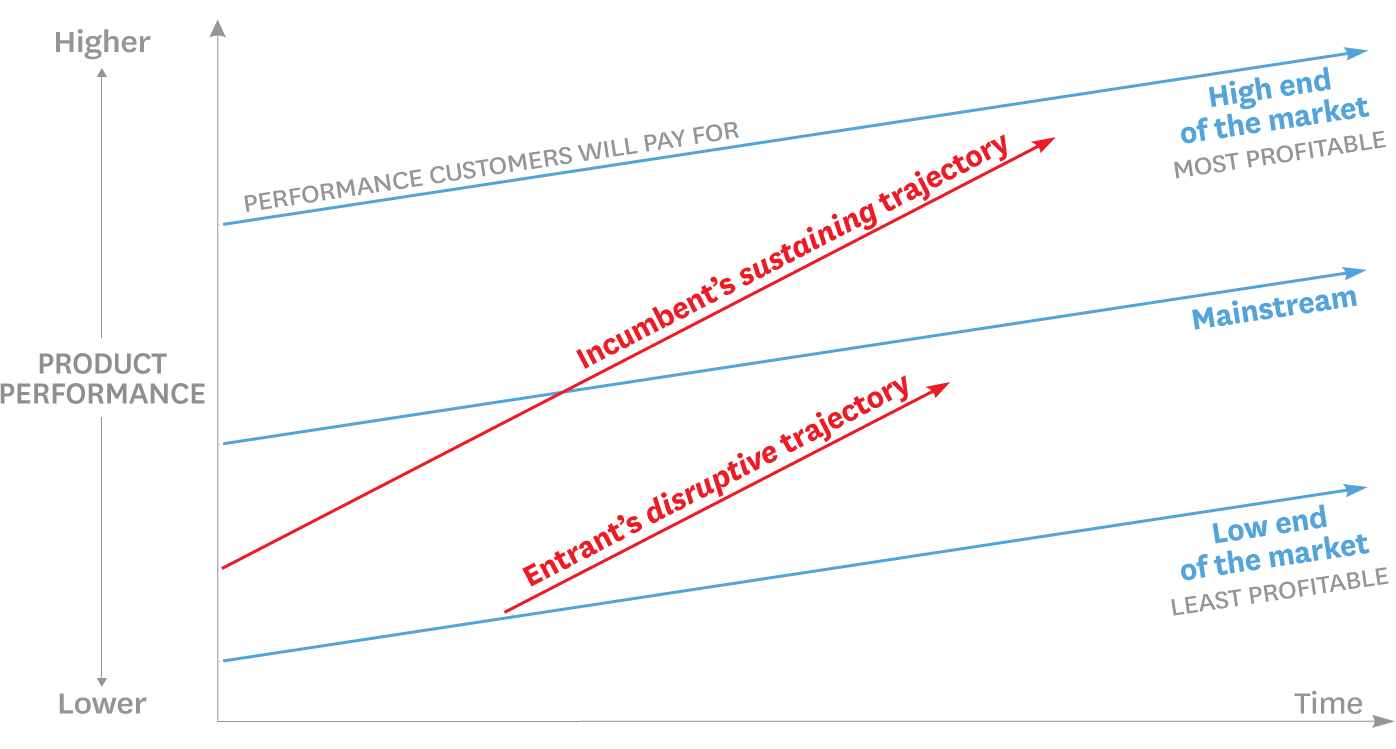
\includegraphics[width=0.9\textwidth]{big-model.png}
    \caption{Model of disruptive innovation \citep{Christensen2015}.}
    \label{fig:graph1}
\end{figure}

The rise of the low cost carriers like Ryanair is often called disruptive innovation.
But do these elements hold up when applied to Ryanair.


\subsection{The Flight Industry}


The incumbents provide food and unlimited drinks on their flights, allocated seats, generous baggage allowance and overall good service. Flights leave from prime location and main, easy to reach, airports. Flights leave on prime times for a high price. Traditional airlines want to improve their performance. \cite{Christensen97} then continuous to describe how this can be disrupted by newcomers that offer a product of worse quality than the incumbent. Although in the beginning they are not seen as a threat because of the inferior design or performance, it can sometimes turn out to be the reason of big firms failure.

\subsection{Ryanair as an Entrant}

Looking at Ryanair's product, \cite{Barrett} notes that Ryanair dropped customer service items compared to the National European Airlines. No extras on the flight and more seats per aircraft. Another major difference is the airport service, by using secondary airports like London Luton instead of London Heathrow. These smaller airports ask lower landing charges. A third observation by \cite{Barrett} is the fact that tickets are sold directly to the customer not via a travel agent, so the airline does not pay any commission to an intermediary. Kenny Jacobs, Chief Marketing Officer, Ryanair says: "On their first low cost flight in 1995 customers paid in cash, which was collected in a bucket as customers departed" \citep{ITBberlin}.

An other feature they introduced is the use of a single air craft of the same specification, which means cheaper in maintenance, less training and every pilot can fly any aircraft in the fleet and the engineers only need to know one type of aircraft. They also save by buying interior, equipment and parts in bulk \citep{Kangis}.

Instead of entering the regular market the Low Cost Airlines looked for new markets at the fringe. This is consistent with
\cite{Christensen97} first element.

\subsection{National Airlines Overshoot the Market}
\label{national}

The main airlines kept doing what they do best and maybe even overshoot the mainstream market by adding more and more 'frills'. \cite{Droege} describes it as value-added attributes, like food and drinks that become standard for mainstream customers. But more new customers enter the market and start flying with low cost carries like Ryanair, their market-share grew. These new travellers talked about this 'good enough' flight and the regular existing market, including business travellers, heard about it and took an interest in these 'cheaper' but good enough flights \citep{TiddBessant}.

As explained by \cite{Christensen2015} the next step would be that the incumbent overshoots the target and the entrants move into
the mainstream market. It is interesting to see this might have been the case at the start of the millennium, but in the following years the incumbent reacted. Still providing leg space and free food and drinks for the demanding customer in Business and, if they offer, in
First Class. The Economy Class traveller can fly cheaper and gets less "frills'. In his article "End of the free lunch?"
\cite{Dennis} argues that the European National airlines adopted many of the low cost mechanisms of the low cost carriers. For
example BA started operating point-to-point routes and making use of regional airports to do so. They added cheaper fares with more
conditions and flexible fares for a higher price. At the time when \cite{Dennis} wrote this article lunches were still free. Since the beginning of 2017 BA out sourced the catering to Marks \& Spencer \citep{Calder}. So it is sufficient to say they did not overshoot the mainstream.


\subsection{Ryanair Moving into Mainstream?}
\label{limits}


With fare reduction Ryanair entered the fringe market in the mid nineties, but soon this attracted more 'regular' travellers as well and not only because of the 'good enough' flights. Additionally, there was also improvements in the service that attracted people. According to \cite{Barrett} Ryanair looses less luggage and they excel in punctuality when it comes to arrival times. On these service levels they score better than national carriers like BA or Air France in 2004. He \citep{Barrett} then continues to explain that this is due to the fact that Ryanair offers a simple product, no connecting flights and uses smaller airports, which makes it easier to meet these levels of service. Furthermore the secondary airports have other benefits like shorter walking distance and less congestion at the border control and check in.


Low cost carriers managed to increased their market share as Figure \ref{fig:graph2} illustrates. So even though the traditional airlines reacted as described by \citep{Dennis} the low cost carriers share of total flights grew from 19\% in 2007 to 30\% in 2016, whereas the traditional carriers, market segment decreased between 2007 and 2016 to 51 \%. From the low cost carriers Ryanair is responsible for the biggest share with 22\% \citep{Eurocontrol2017}

\begin{figure}[h!]
    \centering
    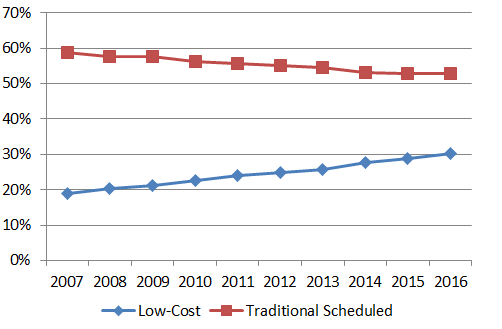
\includegraphics[width=0.9\textwidth]{evolution-lcc-vs-tradsched.png}
    \caption{Evolution of low-cost segment vs traditional scheduled segment \cite{Eurocontrol2017}.}
    \label{fig:graph2}
\end{figure}

\citep{Christensen2015} uses the case of Uber to further explain how to apply the model for disruptive innovation correctly. "Uber has quite arguably been increasing the total demand - that's what happens when you develop a better, less-expensive solution to a widespread customer need" \citep[p. 4]{Christensen2015}. He then continues that disrupters are not mainstream until increase their quality. Looking at Ryanair it is fair to say that they did increase their share of flights but the total number of flights increased as well \citep{Eurocontrol2018} but they have not improved their quality or have been sustaining their innovation into mainstream. The opposite seems true as \citep{Barrett} writes, the demand for cheap flights like Ryanair will probably remain high as long as the fare price is low and Ryanair stays on the trajectory of cutting cost and not engage in expensive projects like new logo's and fancy headquarters. \cite{Eurocontrol2018} identifies low cost carriers have helped traffic grow and also that some are trying to penetrate the long-haul market. To offer these long-haul flights for a cheaper fare is harder to achieve because of operating long-haul flights is more expensive when it comes to aircraft, fuel and crew. They loose the cost effective advantage. So there is no convincing evidence they moved completely into the mainstream market


\subsection{Incumbent Can Not React}
\label{reaction}

Lastly to fit all the elements of the disruptive innovation \cite{Christensen97} claims incumbents can not react because of their existing customers and shareholders who do not allow them to offer an inferior product.
Be that as it may, an anonymous expert in \cite{King} explains the barrier to react in the case of the airline industry is a structural barrier. For competing with a low-cost-carrier on the same business model, the airline would need new aircrafts, workers, airports, gates etcetera and the best response is not to adapt.

As explained in earlier in 'National Airlines Overshoot the Market', adapting is what the main airlines eventually did by copying what worked for the traditional airlines. For example, online check in, booking and less 'frills' for the less demanding, price conscious, customers. At the same time the national carriers keep their focus on their existing market. Which is also what \cite{Christensen2015} recommend, incumbents should still focus on the mainstream and high-end  market, there is still a big profit to be made.


\section{Conclusion}

Although the rise of Ryanair has elements of disruptive innovation it does not fit the model completely. Ryanair as a low cost carrier began as a new entrant in airline business. They started at the fringe, expanded and took passengers from the mainstream on board and grew their market share. The incumbents like BA have overshoot their customer needs maybe a little on short-haul flights where the extras were not necessary. Travellers moved to the cheaper flights, companies like Ryanair were offering.

Ryanair however has, instead of sustaining their product and adding quality to really move into mainstream, set their goal to keep costs low and kept their fares unbundled, charging people for extras. In other words they are staying in the lower end of the market and if they are in the mainstream it is only on short-haul flights. The incumbent on the other side adapted the new, low cost, business model where possible. While at the same time keeping their more demanding and more profit making customers.

\cite{Christensen2015} explain there are a couple of points that are overlooked in using the model of disruptive innovation. They state it is a process and incumbents can be creative in the defence and that incumbent do not need to respond but should continue to provide for their core customers.

The incumbents did not fail and at this moment the business models both survive next to each other.The future will tell if the incumbent fail and the entrants, like Ryanair, will move into the mainstream.

\cite{Diaconu}, recommends Ryanair to start flying from the main airports to get hold of more travellers and business travellers in particular. In their report \cite{Eurocontrol2018} describes how low cost carriers attempt to penetrate the long haul market. If Ryanair succeeds in these and other changes they would fit the model better. But as \cite{Christensen2015} warns the main airlines might be creative and out smart the low cost carriers like Ryanair.




%% disable some things
\renewcommand{\textbf}{}
\renewcommand{\bf}{}
\bibliography{biblio}{}
\end{document}
